\documentclass{article}
\usepackage{tikz}
\usetikzlibrary{shapes}

% Figure to learn the tikz-enviroment a bit better
% Based on the very informative but really really
% badly colored figure shown in a lecture about
% neutron moderation

% Some variables

\newcommand\neutronRadius{0.1} % Do I have to use camel-case?

\begin{document}

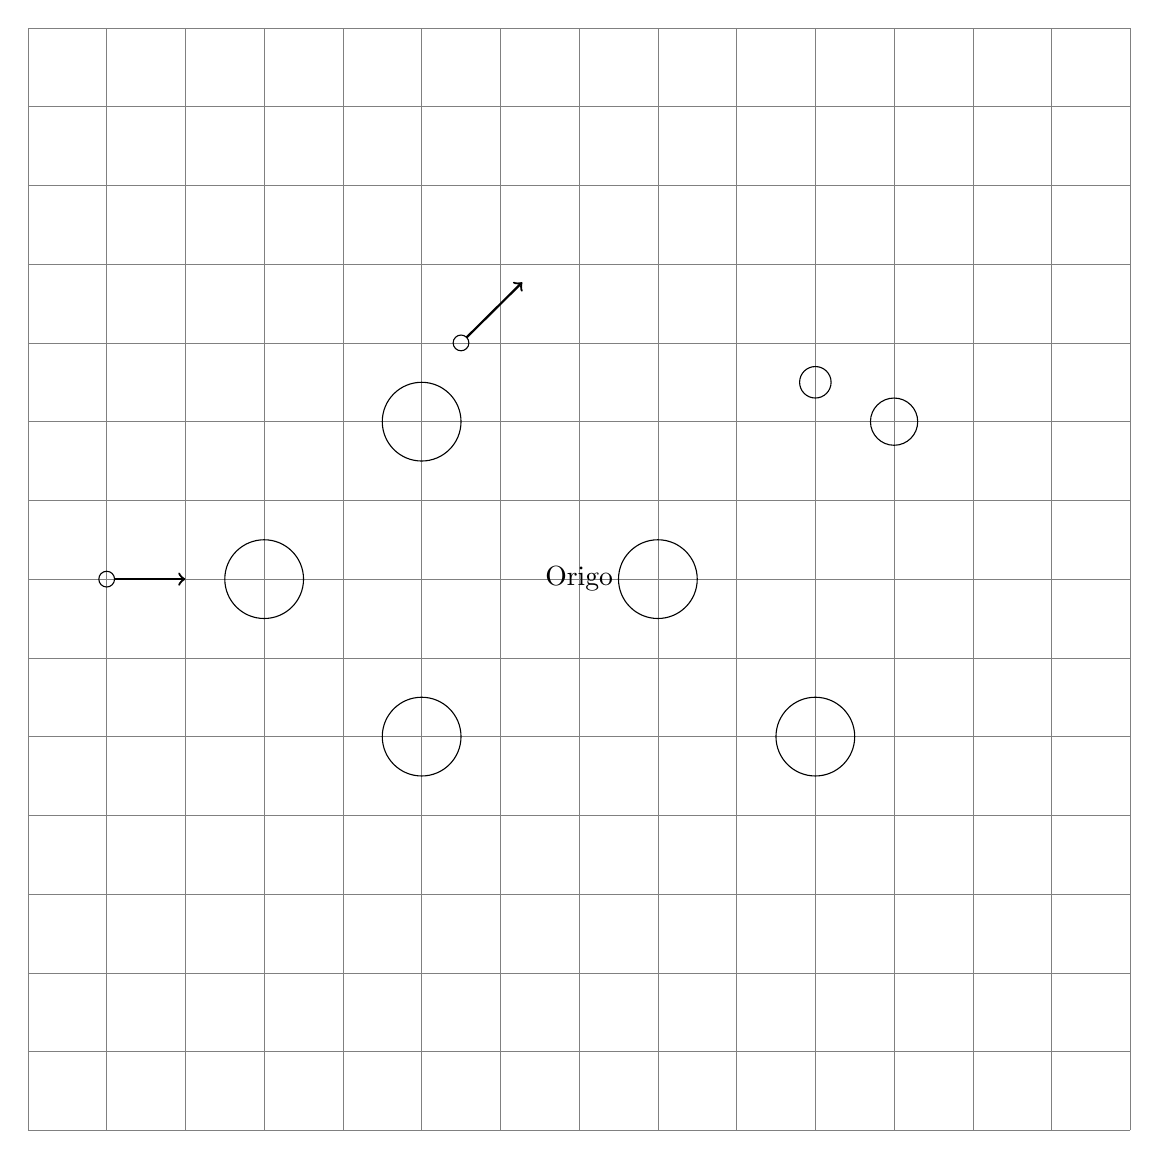
\begin{tikzpicture}
    \draw [step = 1cm, gray, very thin] (-7, -7) grid (7,7); % Grid

    %\clip (-0.1, -0.2) rectangle (1.1, 0.75);
    \draw (1,0) circle [radius = 0.5cm];

    \draw (0,0) node {Origo};

    \draw (-4,0) circle [radius = 0.5cm];
    \draw (-2,2) circle [radius = 0.5cm];
    \draw (-2,-2) circle [radius = 0.5cm];
    \draw (3,-2) circle [radius = 0.5cm];
    
    \draw (3,2.5) circle [radius = 0.2cm];
    \draw (4,2) circle [radius = 0.3cm];


    \draw (-6.0,0) circle [radius = 0.1cm];
    \draw [->, thick] (-5.9,0) -- (-5, 0);
    
    \draw (-1.5,3) circle [radius = 0.1cm];
    \draw [->, thick] (-1.429,3.07) -- (-0.722, 3.77);

\end{tikzpicture}

\end{document}
